\section{Результаты}
\begin{figure}[H]
	\center{\includegraphics[width=0.8\linewidth]{images/input\_data}}
	\caption{Исходные выборки}
	\label{fig:input_data}
\end{figure}
\begin{figure}[H]
	\center{\includegraphics[width=0.8\linewidth]{images/data1\_interval}}
	\caption{"Обинтерваленные"  значения первой выборки}
	\label{fig:data1_interval}
\end{figure}
\begin{figure}[H]
	\center{\includegraphics[width=0.8\linewidth]{images/data1\_fixed}}
	\caption{Линейная регрессия для первой выборки}
	\label{fig:data1_fixed}
\end{figure}
\begin{figure}[H]
	\center{\includegraphics[width=0.8\linewidth]{images/w1\_hist}}
	\caption{Гистограмма коэффициентов коррекции для первой выборки}
	\label{fig:w1_hist}
\end{figure}
\begin{figure}[H]
	\center{\includegraphics[width=0.8\linewidth]{images/data1\_const}}
	\caption{"Спрямленные"  значения первой выборки}
	\label{fig:data1_const}
\end{figure}
\begin{figure}[H]
	\center{\includegraphics[width=0.8\linewidth]{images/data1\_hist\_const}}
	\caption{Гистограмма для скорректированной модели данных первой выборки}
	\label{fig:data1_hist_const}
\end{figure}
\begin{figure}[H]
	\center{\includegraphics[width=0.8\linewidth]{images/data2\_interval}}
	\caption{"Обинтерваленные"  значения второй выборки}
	\label{fig:data2_interval}
\end{figure}
\begin{figure}[H]
	\center{\includegraphics[width=0.8\linewidth]{images/data2\_fixed}}
	\caption{Линейная регрессия для второй выборки}
	\label{fig:data2_fixed}
\end{figure}
\begin{figure}[H]
	\center{\includegraphics[width=0.8\linewidth]{images/w2\_hist}}
	\caption{Гистограмма коэффициентов коррекции для второй выборки}
	\label{fig:w2_hist}
\end{figure}
\begin{figure}[H]
	\center{\includegraphics[width=0.8\linewidth]{images/data2\_const}}
	\caption{"Спрямленные"  значения второй выборки}
	\label{fig:data2_const}
\end{figure}
\begin{figure}[H]
	\center{\includegraphics[width=0.8\linewidth]{images/data1\_hist\_const}}
	\caption{Гистограмма для скорректированной модели данных второй выборки}
	\label{fig:data2_hist_const}
\end{figure}
\begin{figure}[H]
	\center{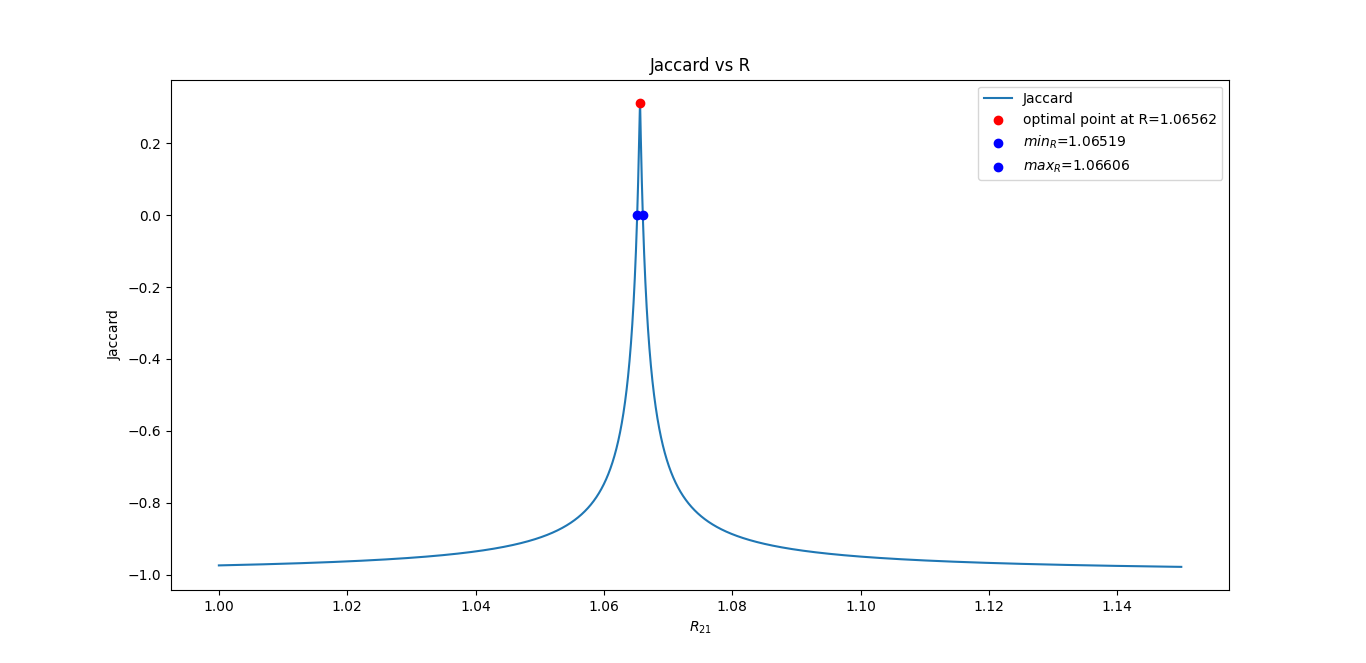
\includegraphics[width=0.8\linewidth]{images/Jaccar}}
	\caption{Коэффициент Жаккара от калибровочного коэффициента}
	\label{fig:jaccar}
\end{figure}